\documentclass{standalone}
\usepackage{pgfplots}
\usetikzlibrary{shapes.geometric, intersections}
\pgfplotsset{compat=1.7}

\begin{document}
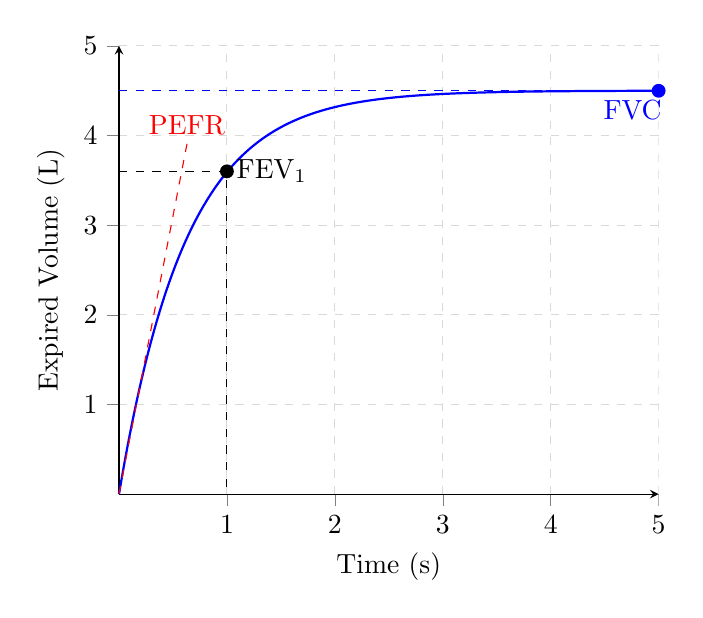
\begin{tikzpicture}
    \begin{axis}[
        axis x line=middle,
        axis y line=middle,
        grid = major,
        grid style={dashed, gray!30},
        xmin=0,     % start the diagram at this x-coordinate
        xmax= 5,    % end   the diagram at this x-coordinate
        ymin= 0,     % start the diagram at this y-coordinate
        ymax= 5,   % end   the diagram at this y-coordinate
        %axis background/.style={fill=white},
	 ylabel near ticks,
	xlabel near ticks,
        xlabel=Time (s),
        ylabel=Expired Volume (L),
        tick align=outside,
        enlargelimits=false,
clip = false]
	

	\addplot[domain=0:5, blue, thick,samples=500] {4.5*(1-exp(-1.6*x))} node[circle,fill=blue,inner sep=0pt,minimum size=5pt, pos=1]{};
	\draw [blue, thin, dashed] (axis cs: 0,4.5) -- (axis cs: 4.4,4.5) node[below right]{FVC};
	\draw [black, thin, dashed] (axis cs: 0,3.6) -- (axis cs: 1, 3.6) node[circle,fill=black,inner sep=0pt,minimum size=5pt]{} node[right]{FEV\textsubscript{1}} -- (axis cs: 1, 0);

	\addplot[domain=0:0.63, red, thin, dashed] {6.2*x} node[above]{PEFR};





\end{axis}

\end{tikzpicture} 
\end{document}